\documentclass{article}
\usepackage[utf8]{inputenc}
\usepackage{graphicx}
\usepackage{fullpage}
\usepackage{multicol}
\usepackage{color}

\setlength{\columnseprule}{2pt}
\def\columnseprulecolor{\color{green}}

\begin{document}
\subsection{Persona 1}
\begin{figure}[h!]
    \centering
    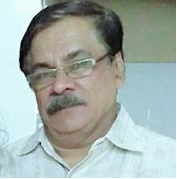
\includegraphics{picture}
\end{figure}
\begin{multicols}{2}[]
\noindent
\textbf{Name:} Prof. Bhupendra Kesaria \\
\newline
\textbf{Email:} bhupendra.kesaria@upgcm.ac.in \\
\newline
\textbf{Gender:} Male \\
\newline
\textbf{Age:} 59 \\
\newline
\textbf{Profession:} Professor \\
\newline
\textbf{Skill level:} Expert \\
\newline
\textbf{User story:} Prof. Bhupendra Kesaria has cleared National Eligibility Test (NET) in Computer Science in the year 2012. He has done Masters in Computer Applications from Indira Gandhi National Open University(IGNOU). He has done Advanced Diploma in Computer Applications from IGNOU. He has done his Bachelors in Computer Applications from IGNOU. Prof. Kesaria has worked in industry with companies like Khatau Group of Companies, Avnet Technologies. He had been a consultant to companies like Mail Order Solutions Pvt Ltd and Evergreen Engineering Company. He has 13 years of teaching experience. He has an industry experience of 12 years. He has taught in Universities like IGNOU,ICFAI,Manipal,ITM,TMU and in National Institute of Fashion Technology. \\
\columnbreak
\newline
\textbf{Wishes: } 
\begin{enumerate}
    \item He want to improve the teaching pattern for mathematics.
    \item He wants to save time and able to teach efficiently.
    \item He wishes to educate more about vedic math.
\end{enumerate}
\textbf{Motivation:}
\begin{enumerate}
    \item He want to start his own coaching center.
    \item A coaching class which emphasises more on natural ways of calculating and computing.
    \item His goals consists of globalization of his coaching center.
\end{enumerate}
\textbf{Pain Points:}
\begin{enumerate}
    \item He does not like that a student uses calculator more often rather than using his/her brain.
    \item He gets annoyed when student uses wrong formula for a problem.
\end{enumerate}
\end{multicols}
\newpage
\subsection{Persona 2}
\begin{figure}[h!]
    \centering
    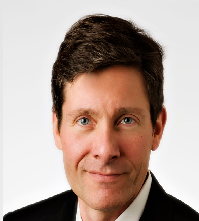
\includegraphics{picture2.jpg}
\end{figure}
\begin{multicols}{2}[]
\noindent
\textbf{Name:} Alexandros Mavrias \\
\newline
\textbf{Email:} a\_mavrias@hotmail.com \\
\newline
\textbf{Gender:} Male \\
\newline
\textbf{Age:} 37 \\
\newline
\textbf{Profession:} Investment Analys \\
\newline
\textbf{Skill level:} Expert \\
\newline
\textbf{User story:} Alexandros has done B.Com. and MBA from McGill university. He has created financial models to determine the feasibility of joint ventures with international partners and capital investment projects for the company’s network of global training centers. He performed fundamental analysis of US and Latin American companies operating in the financial, energy, material and utility sectors. He has developed financial models to determine the intrinsic value of companies, including sensitivity and scenario analysis \\
\columnbreak
\newline
\textbf{Wishes: } 
\begin{enumerate}
    \item He wants to create more functional investment models for customers.
    \item Alexandros wishes to continue serving to customers for better investment plans.
\end{enumerate}
\textbf{Motivation:}
\begin{enumerate}
    \item He want to make history by creating new investment plans to benefit the company as well as the customer.
    \item "Double up the money" is his dream project where he wants to double the client's money in as short time as possible.
\end{enumerate}
\textbf{Pain Points:}
\begin{enumerate}
    \item He does not like when for small investment also he needs to calculate and do lot of math.
    \item He does not like the lack of options that are provided by Business calculator.
\end{enumerate}
\end{multicols}
\end{document}